% Chapter 2, Topic _Linear Algebra_ Jim Hefferon
%  http://joshua.smcvt.edu/linearalgebra
%  2001-Jun-11
\topic{Kristal}
\index{kristal|(}
Semua orang pernah memperhatikan bahwa garam dapur\index{garam}
berbentuk kubus-kubus kecil.
\begin{center}
  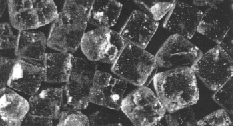
\includegraphics[height=1.25in]{vs/pix/salt.jpg} %1.25in tall
\end{center}
Keteraturan di bagian luar ini muncul dari keteraturan di bagian dalam\Dash 
susunan atom-atomnya juga berbentuk kubus,
kubus-kubus ini tertumpuk dalam baris dan kolom yang rapi, dan permukaan
garam cenderung hanya berupa lapisan terluar kubus-kubus tersebut.
Satu kubus atom ditunjukkan di bawah ini.
Garam adalah natrium klorida; bola-bola kecil yang ditampilkan adalah
natrium, sedangkan bola-bola besar adalah klorida.
Untuk menyederhanakan gambar, hanya natrium dan klorida pada sisi depan, 
atas, dan kanan yang ditampilkan.
\begin{center}
  \includegraphics{vs/mp/ch2.1}
\end{center}
Butiran-butiran garam yang kita lihat di atas 
memiliki banyak pengulangan satuan dasar ini. 
Padatan, seperti garam dapur, 
yang memiliki struktur internal teratur disebut \definend{kristal}.

Kita dapat membatasi perhatian pada sisi depan.
Di sana terdapat persegi yang berulang berkali-kali sehingga membentuk
kisi atom.
\begin{center}
  \includegraphics{vs/mp/ch2.9}
\end{center}
Panjang sisi setiap sel persegi 
sekitar $3.34$~\AA ngstrom
(satu \AA ngstrom sama dengan $10^{-10}$~meter).
Ketika kita ingin merujuk pada atom-atom di dalam kisi, 
angka tersebut tidak praktis, sehingga 
kita menggunakan panjang sisi persegi sebagai satuan.
Dengan kata lain, secara alami kita menggunakan basis ini.
\begin{equation*}
  \sequence{\colvec{ 3.34 \\ 0},\colvec{0 \\ 3.34}}
\tag*{}\end{equation*}
Sekarang, misalnya, kita dapat menyatakan atom di kanan atas gambar kisi
di atas sebagai $3\vec{\beta}_1+2\vec{\beta}_2$, alih-alih sebagai
$10.02$~\AA ngstrom ke kanan dan $6.68$~ke atas.

Kristal lain yang dijumpai dalam kehidupan sehari-hari adalah isi pensil.
Bahan itu adalah \definend{grafit},\index{grafit} 
yang terbentuk dari atom-atom karbon dengan susunan seperti ini.
\begin{center}  %graphite
  \includegraphics{vs/mp/ch2.10}
\end{center}
Ini adalah satu bidang grafit yang disebut \definend{grafena}.
Sepotong grafit terdiri atas banyak bidang semacam ini yang berlapis-lapis.
Ikatan kimia di antara bidang-bidang tersebut jauh lebih lemah daripada
ikatan di dalam setiap bidang. Hal ini menjelaskan mengapa pensil dapat
digunakan untuk menulis\Dash grafit dapat tergeser sehingga bidang-bidangnya
terlepas dan tertinggal di atas kertas.

Kita dapat memperoleh satuan panjang yang praktis dengan
menguraikan cincin heksagonal menjadi tiga daerah yang merupakan hasil rotasi
dari \definend{sel satuan} ini.\index{kristal!sel satuan} 
\begin{center}  %graphite
  \includegraphics{vs/mp/ch2.11}
\qquad\qquad
\includegraphics{vs/mp/ch2.12}
\end{center}
Vektor-vektor yang membentuk sisi-sisi
sel satuan tersebut menghasilkan basis yang praktis.
Panjang sisi bawah dan sisi miringnya adalah $1.42$~\AA ngstrom, 
sehingga
\begin{equation*}
  \sequence{\colvec{1.42 \\ 0}, \colvec{0.71 \\ 1.23}}
\tag*{}\end{equation*}   
merupakan basis yang baik.

Kristal lain yang umum dikenal dan terbentuk dari karbon adalah
intan.\index{intan}
Seperti garam dapur, intan tersusun dari kubus-kubus, tetapi struktur di
dalam setiap kubus lebih rumit. 
Selain atom karbon pada setiap sudut,
\begin{center}
  \includegraphics{vs/mp/ch2.13}
\end{center}
terdapat atom karbon di tengah setiap sisi. 
\begin{center}
  \includegraphics{vs/mp/ch2.14}
\end{center}
(Agar atom karbon baru pada sisi terlihat jelas, 
atom karbon pada sudut digambarkan sebagai titik.)
Terdapat pula empat atom karbon lain di dalam kubus, 
dua pada seperempat jarak ke atas dari dasar 
dan dua pada seperempat jarak ke bawah dari bagian atas.
\begin{center}
  \includegraphics{vs/mp/ch2.15}  
\end{center}
(Seperti sebelumnya, atom karbon yang telah ditampilkan digambarkan di sini
sebagai titik.)
Panjang setiap rusuk kubus adalah $2.18$~\AA ngstrom. 
Jadi, basis alami untuk menyatakan letak atom-atom karbon
dan ikatan di antaranya adalah sebagai berikut.
\begin{equation*}
  \sequence{\colvec{2.18 \\ 0 \\ 0}, 
            \colvec{0 \\ 2.18 \\ 0}, 
            \colvec{0 \\ 0 \\ 2.18}}
\tag*{}\end{equation*}   

Contoh-contoh di sini menunjukkan bahwa
struktur kristal cukup rumit sehingga diperlukan suatu sistem yang teratur
untuk menyatakan letak atom-atom dan cara atom-atom tersebut berikatan secara
kimia.
Salah satu alat untuk pengaturan itu adalah basis yang praktis.
Penerapan basis ini sederhana, tetapi memperlihatkan suatu konteks ilmiah
tempat gagasan tersebut muncul secara alami.
% The work in this chapter just takes this simple idea and develops it.

\begin{exercises}
  \item 
    Berapa banyak daerah dasar pada satu sisi sebutir garam? 
   (Dengan penggaris, kita dapat memperkirakan bahwa sisi tersebut berbentuk
   persegi dengan panjang sisi $0.1$~cm.)
   \begin{answer}
     Setiap satuan dasar berukuran $3.34\times 10^{-8}$~cm, sehingga terdapat
     sekitar $0.1/(3.34\times 10^{-8})$ satuan semacam itu.
     Hasilnya adalah $2.99\times 10^{6}$, jadi terdapat kira-kira
     $3,000,000$ (tiga juta) daerah.
   \end{answer}
  \item 
    Pada gambar grafit, bayangkan bahwa kita tertarik pada suatu titik 
    yang terletak $5.67$~\AA ngstrom ke kanan dan $3.14$~\AA ngstrom ke atas
    dari titik asal.
    \begin{exparts}
      \partsitem Nyatakan titik tersebut dalam basis yang diberikan
        untuk grafit.
      \partsitem Titik ini berjarak berapa banyak bentuk heksagonal dari
        titik asal? 
      \partsitem Nyatakan titik tersebut dalam basis kedua,
        dengan vektor basis pertama tetap sama, sedangkan vektor kedua 
        tegak lurus terhadap yang pertama (mengarah ke atas bidang) dan
        memiliki panjang yang sama.
    \end{exparts} 
    \begin{answer}
      \begin{exparts}
        \partsitem Kita menyelesaikan
          \begin{equation*}
            c_1\colvec{1.42 \\ 0}+c_2\colvec{0.71 \\ 1.23}
              =\colvec{5.67 \\ 3.14}
            \quad\implies\quad
            \begin{linsys}{2}
              1.42c_1  &+  &0.71c_2  &=  &5.67  \\
                       &   &1.23c_2  &=  &3.14
            \end{linsys}
          \tag*{}\end{equation*}
          sehingga diperoleh $c_1\approx 2.72$ dan $c_2\approx 2.55$.
        \partsitem Berikut adalah letak titik tersebut di dalam kisi.
          Pada gambar di sebelah kiri, dua vektor basis $\vec{\beta}_1$ dan
          $\vec{\beta}_2$ ditumpangkan pada sel satuan, 
          bersama sebuah kotak yang menunjukkan pergeseran sebesar 
          $2.72\vec{\beta}_1+2.55\vec{\beta}_2$.
          Gambar di sebelah kanan menunjukkan letaknya di dalam kisi kristal,
          dengan sudut kiri bawah heksagon di kiri bawah sebagai titik asal. 
          \begin{center}  %graphite
            \includegraphics{vs/mp/ch2.17}
            \qquad
            \includegraphics{vs/mp/ch2.18}
       \end{center}
       Jadi, titik ini berada dua kolom heksagon ke kanan dan  
       satu heksagon ke atas.
      \partsitem Basis kedua ini
          \begin{equation*}
            \sequence{\colvec{1.42 \\ 0},\colvec{0 \\ 1.42}}
          \tag*{}\end{equation*}
          mempermudah perhitungan
          \begin{equation*}
            c_1\colvec{1.42 \\ 0}+c_2\colvec{0 \\ 1.42}
              =\colvec{5.67 \\ 3.14}
            \quad\implies\quad
            \begin{linsys}{2}
              1.42c_1  &   &         &=  &5.67  \\
                       &   &1.42c_2  &=  &3.14
            \end{linsys}
          \tag*{}\end{equation*}
          (kita memperoleh $c_2\approx 2.21$ dan $c_1\approx 3.99$), tetapi
          basis ini tampaknya tidak banyak berkaitan dengan struktur fisik
          yang sedang kita pelajari. 
      \end{exparts}
    \end{answer}
  \item 
    Berikan letak atom-atom di dalam kubus intan, baik
    dalam basis tersebut maupun dalam \AA ngstrom.
    \begin{answer}
      Dalam basis tersebut, letak atom-atom sudut adalah
      $(0,0,0)$, $(1,0,0)$, \ldots, $(1,1,1)$.
      Letak atom-atom sisi adalah $(0.5,0.5,1)$, $(1,0.5,0.5)$,
      $(0.5,1,0.5)$, $(0,0.5,0.5)$, $(0.5,0,0.5)$, dan $(0.5,0.5,0)$.
      Letak atom-atom pada seperempat jarak ke bawah dari bagian atas
      adalah $(0.75,0.75,0.75)$ dan $(0.25,0.25,0.25)$. 
      Atom-atom pada seperempat jarak ke atas dari dasar
      berada di $(0.75,0.25,0.25)$ dan $(0.25,0.75,0.25)$. 
      Konversi ke \AA ngstrom dapat dilakukan dengan mudah.
    \end{answer}
  \item 
    Soal ini menggambarkan cara menghitung 
    dimensi sel satuan dari bentuk kristalisasi 
    suatu zat 
    (\cite{Ebbing}, hlm.~462).
    \begin{exparts}
      \partsitem Ingat bahwa terdapat $6.022\times 10^{23}$ atom dalam satu mol
        (ini adalah bilangan Avogadro).
        Dengan menggunakan fakta tersebut dan fakta bahwa platina memiliki
        massa $195.08$ gram per mol, hitunglah massa setiap atom.
      \partsitem Platina mengkristal dalam kisi kubik berpusat muka
        dengan atom pada setiap titik kisi;
        artinya, bentuknya seperti gambar tengah kristal intan di atas.
        Tentukan banyaknya atom platina per sel satuan
        (petunjuk:~jumlahkan fraksi-fraksi atom platina yang berada di dalam
        satu sel).
      \partsitem Berdasarkan hasil tersebut, tentukan massa satu sel satuan.
      \partsitem Kristal platina memiliki 
        massa jenis $21.45$ gram per sentimeter kubik.
        Dengan menggunakan nilai ini dan massa satu sel satuan, hitunglah
        volume satu sel satuan.
      \partsitem Tentukan panjang setiap rusuk.
      \partsitem Uraikan sebuah basis tiga dimensi yang alami.
    \end{exparts}
    \begin{answer}
      \begin{exparts}
        \partsitem $195.08/(6.022\times 10^{23})=3.239\times 10^{-22}$
        \partsitem Setiap atom platina di tengah suatu sisi terbagi di antara
          dua kubus, sehingga sejauh ini terdapat $6/2=3$ atom.
          Setiap atom pada sudut terbagi di antara delapan kubus, sehingga 
          terdapat tambahan $8/8=1$~atom; jadi jumlahnya $4$.
        \partsitem $4\cdot 3.239\times 10^{-22}=1.296\times 10^{-21}$
        \partsitem $1.296\times 10^{-21}/21.45=6.042\times 10^{-23}$
           sentimeter kubik
        \partsitem $3.924\times 10^{-8}$ sentimeter.
        \partsitem 
            $\sequence{\colvec{3.924\times 10^{-8} \\ 0 \\ 0},
                       \colvec{0 \\ 3.924\times 10^{-8} \\ 0},
                       \colvec{0 \\ 0 \\ 3.924\times 10^{-8}}}$
      \end{exparts}
    \end{answer}
\end{exercises}
\index{kristal|)}
\endinput
